\chapter{Functional analysis}
\label{ch:functional_analysis}
This section aims to give a detailed higher level overview of the overall real-world application of the proposed solution.

\begin{figure}[h!]
    \centering
    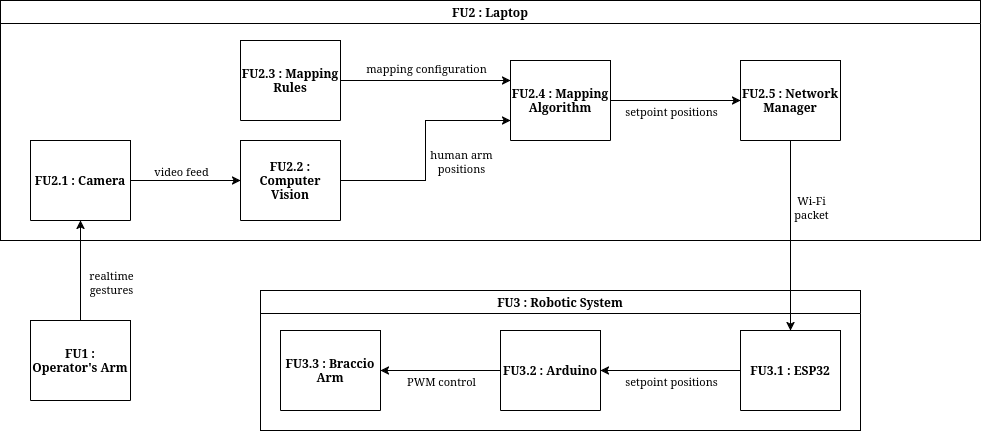
\includegraphics[width=1\textwidth]{graphics/system_block_diagram.png}
    \caption{System Block Diagram}
\end{figure}

\textbf{FU1,} the operator's arm, serves as the primary input to the system. Its positions ultimately determine the setpoint for the Braccio arm (FU3.3).

\textbf{FU2,} the student's laptop, serves as the interface through which the operator's arm positions get captured, interpreted, and wirelessly sent to the robotic system (FU3). The primary components are: a camera, Wi-Fi antenna, and a software pipeline. \textit{\textbf{FU2.1,}} the laptop's camera, captures the operator's arm's gestures/positions, and feeds this to the computer vision algorithm (FU2.2). \textit{\textbf{FU2.2,}} the computer vision algorithm, processes the camera's video feed, and models the operator's arm's position. FU2.2 and FU2.1 will likely be handled by a singular open source solution. \textit{\textbf{FU2.3,}} the mapping rules, is a file and/or data structure that specifies how the human arm's positions relate to the Braccio arm's positions, in a high-level of abstraction. This is the method that engineers would use to configure the mapping in other projects as well. \textit{\textbf{FU2.4,}} the mapping algorithm, takes the operator's arm's positions, as well as the mapping configuration, to determine the best-approximation setpoints for the Braccio arm (FU3.3). \textit{\textbf{FU2.5,}} the network manager, converts the setpoints into data packets and sends them to the ESP32 (FU3.1) over Wi-Fi.

\textbf{FU3}, the robotic system, is the remote actuator that is intended on being controlled, along with assisting peripherals. \textit{\textbf{FU3.1,}} the ESP32, receives the Wi-Fi data packets, and gives them to the Arduino (FU3.2) over a serial communication protocol. The protocol will likely be UART, since there aren't multiple slave devices to communicate with, and full-duplex communication is not necessary. \textit{\textbf{FU3.2,}} the Arduino, asynchronously receives setpoints from the ESP32 (FU3.1), while controlling the Braccio arm (FU3.3) with PWM signals (the Braccio uses servo motors). \textit{\textbf{FU3.3}}, the Braccio arm, is the actuator that's being controlled by the user. Its effective accuracy and speed is how the system's overall performance is measured.
